\myChapter{Estensione della libreria FACPL}
\label{cap:estensione_libreria}
Il linguaggio \ac{FACPL} è supportato da una libreria Java. Per supportare l'estensione proposta
abbiamo esteso questa libreria. Per ovvi motivi verranno mostrate solo alcune parti delle modifiche effettuate, ma 
il codice completo si può comunque trovare su GitHub all'url \url{https://github.com/andreamargheri/FACPL}.\par
In Sezione~\ref{sec:imp_stato} è presentata l'implementazione in Java dello stato e degli attributi di stato. Lo stato ha richiesto anche l'implementazione di altre componenti come le funzioni per modificare gli attributi e l'estensione del \ac{PEP}.
Nella Sezione~\ref{sec:estensione_politiche} è trattata l'estensione delle politiche. In particolare si parla di come è stato possibile 
effettuare comparazioni su attributi di stato e di come sono state estese le obligation.
In Sezione~\ref{sec:plugin_eclipse} viene mostrato come è stato esteso il plugin di \ac{FACPL} per supportare le nuove estensioni.
Infine, in Sezione~\ref{sec:implementazione_esempi}, vengono presentati in Java i case study già proposti in Capitolo \ref{cap:usagecontrolfacpl} e
\ref{cap:accessControl}
\section{Implementazione Stato}
\label{sec:imp_stato}
Il primo passo per estendere la libreria è stato la creazione di uno \status, che è modellato da una semplice classe 
di cui ne verrà mostrato un pezzo in Codice~\ref{lst:PezzoStatus1}. Il fulcro di questa classe è una Hashmap con key parametrizzata a 
\statusattribute \ e valore corrispondente parametrizzato ad Object. Questa Hashmap associa quindi ad uno \statusattribute\ il suo valore corrispondente.
\myIjava{status.java}{Stralcio della classe Status}{1}{7}{PezzoStatus1}

In Figura~\ref{fig:statusUML.png} è possibile vedere la relazione che intecorre tra lo stato ed i suoi attributi. 
\MyFig{statusUML.png}{Grafico UML delle classi Status e StatusAttribute}{1}{H}
Come si vede dal grafico UML in Figura \ref{fig:statusUML.png} la classe che modella lo stato include altri due metodi non mostrati in Codice~\ref{lst:PezzoStatus1}. Per via del nome assegnatogli i metodi risultano abbastanza autoesplicativi, per questo ne verrà mostrato solo uno in Codice~\ref{lst:PezzoStatus2}.
\myIjava{status.java}{Set Attribute della classe Status}{32}{37}{PezzoStatus2}

\subsection{Status Attribute}
\label{sub:status_attribute}
Uno Status Attribute è un tipo particolare di attributo. Come si può vedere dalla Figura \ref{fig:statusUML.png} per creare questo nuovo tipo è stata estesa una classe già esistente, ovvero quella che rappresenta gli attributi normali.
\myIjava{SA.java}{Classe Status Attribute}{1}{6}{StatusAttribute}
Nel Codice \ref{lst:StatusAttribute} è possibile vedere il costruttore e i campi di questa nuova classe. In aggiunta agli attributi normali è stato aggiunto un Tipo, che può essere:
\begin{itemize}
	\item Int
	\item String
	\item Date
	\item Boolean
	\item Double
\end{itemize}
Il costruttore riceve due parametri: l'ID e il tipo. In questo metodo viene invocato il costruttore della superclasse dove gli viene passata una categoria fissata, ovvero \textit{Status} e l'ID.
\subsection{Funzioni su Status Attribute}
\label{sub:funzioni_status_attribute}
Le funzioni sugli status attribute sono operazioni che ne vanno a modificare il valore. Derivano tutte da un unica interfaccia mostrata in Codice~\ref{lst:IExpressionFunctionStatus.java}, che avrà come unico metodo quello che eseguirà la vera e propria operazione.
\myjava{IExpressionFunctionStatus.java}{Interfaccia per le operazioni}
Dal grafico UML in Figura~\ref{fig:functionarith.png} si vede chiaramente che ci sono due grandi gerarchie di classi, quelle che fanno operazioni sui numeri, e quelle che fanno operazioni sulle stringhe.
Per eseguire un operazione è sufficiente istanziare una classe che estende \textit{StringOperationStatus} o \textit{MathOperationStatus}, e chiamare l'unico metodo definito nell'interfaccia in Codice \ref{lst:IExpressionFunctionStatus.java} passandogli i parametri corretti. La sottoclasse istanziata eredita il metodo \textit{evaluateFunction} dalla superclasse ed implementa il metodo astratto \textit{op}. Il metodo \textit{evaluateFunction} implementato nella superclasse, in base ai parametri che gli vengono passati si fa restituire da una factory, in base al tipo del attributo, il valutatore corretto che passerà a sua volta al metodo astratto \textit{op}. Il valutatore è una classe dove è scritto il codice Java che eseguirà l'operazione vera e propria.
Nel Codice~\ref{lst:addStatus.java} viene mostrata la sottoclasse che si occupa della somma su numeri. Si nota subito che questa è una sottoclasse di \textit{MathOperationStatus} e che implementa solo il metodo \textit{Op}.
\myjava{addStatus.java}{Add Status}
La ragione dietro la verbosità creata dall'utilizzo di un valutatore, oltre che da una moltitudine di classi e sottoclassi, potrebbe sembrare superflua; ciononostante quest'ultima è una scelta lungimirante, in quanto in futuro sarà più agevole implementare nuovi tipi di attributo e relative funzioni su di essi.

\begin{sidewaysfigure}
    \centering
	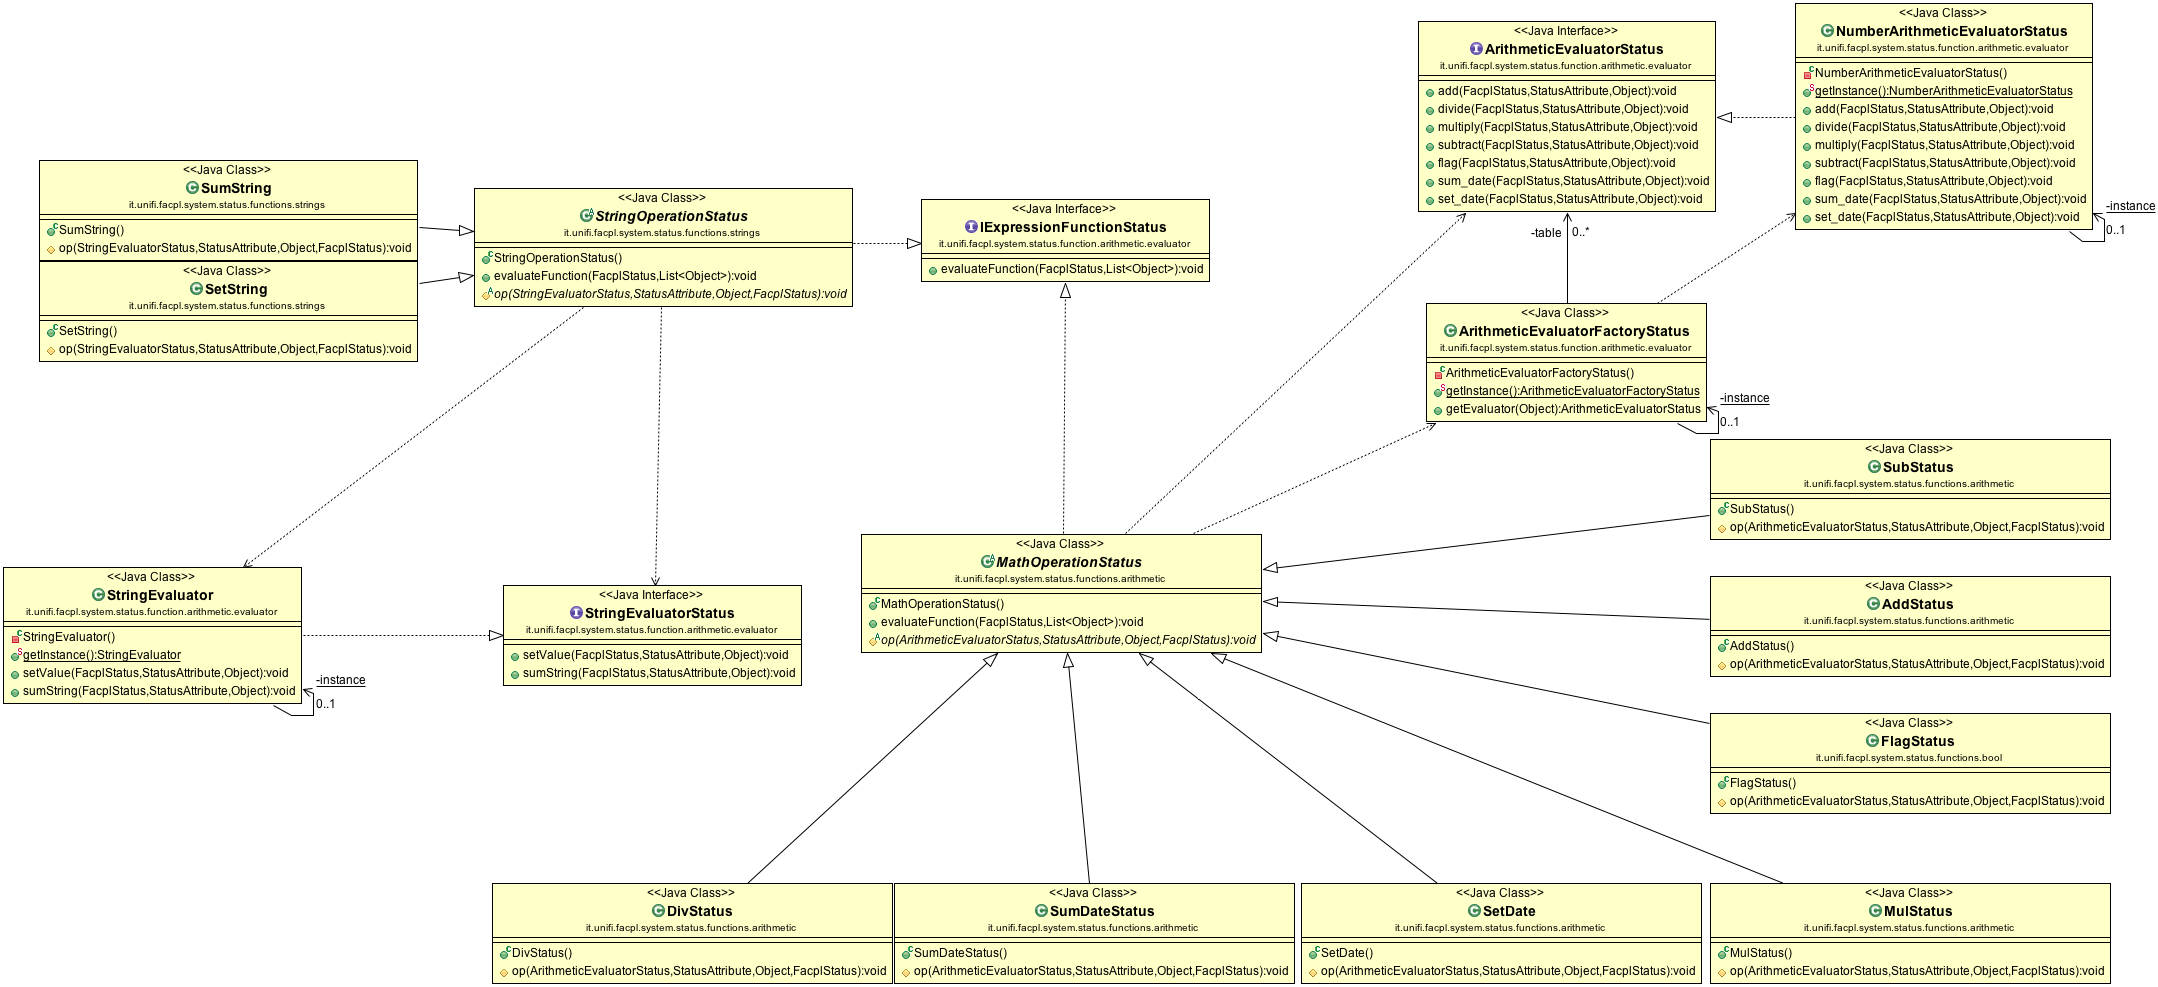
\includegraphics[width=1.0\linewidth]{functionarith.png}
    \caption{Grafico UML per la gerarchia di funzioni aritmetiche}
    \label{fig:functionarith.png}
\end{sidewaysfigure}

\subsection{Estensione del PEP}
\label{sub:estensione_PEP}
La struttura del PEP è rimasta pressoché uguale in quanto non è stato esteso, bensì modificato.
In seguito alla valutazione di una policy il PDP darà una risposta, su questa risposta il PEP dovrà effettuare il suo processo di enforcement.
Durante questo processo vengono valutate le \textit{Obligation} in modo che l'operazione al loro interno sia eseguita; il metodo che effettua questo compito è 
\textit{dischargeObligation}. La modifica ha coinvolto proprio quest'ultimo, in quanto è bastato aggiungere un \textit{else if}, mostrato in Codice~\ref{lst:PEP}, a quelli già presenti.
\myIjava{PEP.java}{Discharge delle Fulfilled Obligation di stato}{102}{106}{PEP}
In questo modo vengono prese in considerazione anche le nuove Obligation Status, quindi ora il PEP, durante il suo processo di enforcement, riuscendo ad eseguire questo nuovo tipo di Obligation potrà modificare lo stato.


\section{Estensione delle politiche}
\label{sec:estensione_politiche}

Le politiche, in seguito all'estensione, vengono valutate basandosi anche sullo stato indi per cui è stato necessario estendere il contesto intorno a cui sono valutate. Come mostrato in Figura~\ref{fig:contextrequest.png} l'estensione del contesto si ottiene mediante la creazione di una nuova classe, a estensione di quella esistente.
\MyFig{contextrequest.png}{Contesto}{0.5}{H}
La nuova classe ContextRequest\_Status contiene lo stato sottoforma di campo privato. L'accesso allo stato è effettuato tramite il metodo getContextRequestValue (Codice~\ref{lst:cxtReq}), che in questa sottoclasse è stato riscritto.
\myIjava{context_request_status.java}{Discharge delle Fulfilled Obligation di stato}{37}{55}{cxtReq}
Questo metodo riceve come parametro un attributo, ed in base al suo tipo andrà a cercarlo nello stato o nell'ambiente.

\subsection{Funzioni di controllo su status}
\label{sub:funzioni_controllo_status}

Il PDP per poter valutare correttamente le richieste deve avere la possibilità di comparare anche questo nuovo tipo di attributi.
Raggiungere quest'obiettivo non è stato difficile in quanto la struttura era già esistente e funzionante, ed essendo i nuovi attributi soltanto un estensione di quelli 
creati in precedenza è stato possibile usarla senza alcun tipo di problema.\par

\MyFig{comparisonUML.png}{Comparatori}{1.2}{H}
Come nel caso delle funzioni di modifica dello stato, la struttura è basata su un factory che ritorna il valutatore corretto in base al tipo su cui deve essere effettuato il confronto.

\subsection{Obligation}
\label{sub:estensione_obligation}
Le \textit{Obligation} sono state estese introducendo un nuovo tipo chiamato \textit{Obligation Status}, questo tipo particolare di \textit{Obligation} servono per andare ad eseguire azioni sullo stato.
Nella libreria sono presenti due tipi fondamentali di \textit{Obligation}, il primo sono quelle a livello sintattico, le seconde, chiamate \textit{FulfilledObligations} sono quelle pronte ad essere valutate. Vediamo adesso come sono state estese quelle a livello sintattico.\\ \par
Per eseguire questa estensione è stato reso necessario un refactoring, per prima cosa è stato astratto tutto il comportamento comune in una superclasse astratta, successivamente è stata creata la nuova classe che modella questo nuovo tipo.
Il refactoring ha coinvolto anche il metodo che si occupa del \textit{Fulfilling} delle \textit{Obligation} in quanto ora deve creare anche questo nuovo tipo, la scelta più ovvia è stata creare un metodo astratto implementato nelle due sottoclassi che viene chiamato dalla superclasse per creare il tipo corretto.
\myIjava{absObl.java}{Parte rifattorizzata del metodo che si occupa del fulfilling}{16}{18}{fulfilabs}
\myIjava{oblStat.java}{CreateObligation nelle status}{17}{24}{createoblstat}
\myIjava{oblNorm.java}{CreateObligation nelle normali}{11}{14}{createoblnorm}
La \textit{Obligation} di stato necessiterà anche di argomenti su cui eseguire l'azione, che le verranno passati in fase di costruzione.\\ \par
Alla fine della valutazione il PDP crea un oggetto di tipo \textit{AuthorisationPDP} che conterrà la decisione e una lista di \textit{FulfilledObligation}, quest'ultime poi andranno al PEP per la loro valutazione. Vediamo ora come sono state implementate.\\ \par
Anche in questo caso è stato necessario un refactoring analogo a quello fatto per le prime.
\myIjava{FulOblStat.java}{Peculiarità della classe FulfilledObligationStatus}{1}{15}{pecfulstat}
Come si può notare, in fase di costruzione, gli verrà passato un oggetto di tipo \textit{IExpressionFunctionStatus} che sarà l'azione che andrà a eseguire sullo stato. Quest'azione andrà realmente ad essere eseguita quando verrà chiamato dal PEP il metodo \textit{evaluateObl}.\\ \par
Il PEP nella fase di enforcement effettua la valutazione delle \textit{Obligation}, in questo caso le modifiche per permettere al sistema di eseguirle sono state minime, è bastato modificare il metodo \textit{DischargeObligation} in modo che quando gli viene passata una \textit{AbstractFulfilledObligation} chiamasse il metodo \textit{evaluateObl} .
\myIjava{PEP.java}{Discharge delle Fulfilled Obligation di stato}{102}{106}{PEP}
\begin{sidewaysfigure}
    \centering
	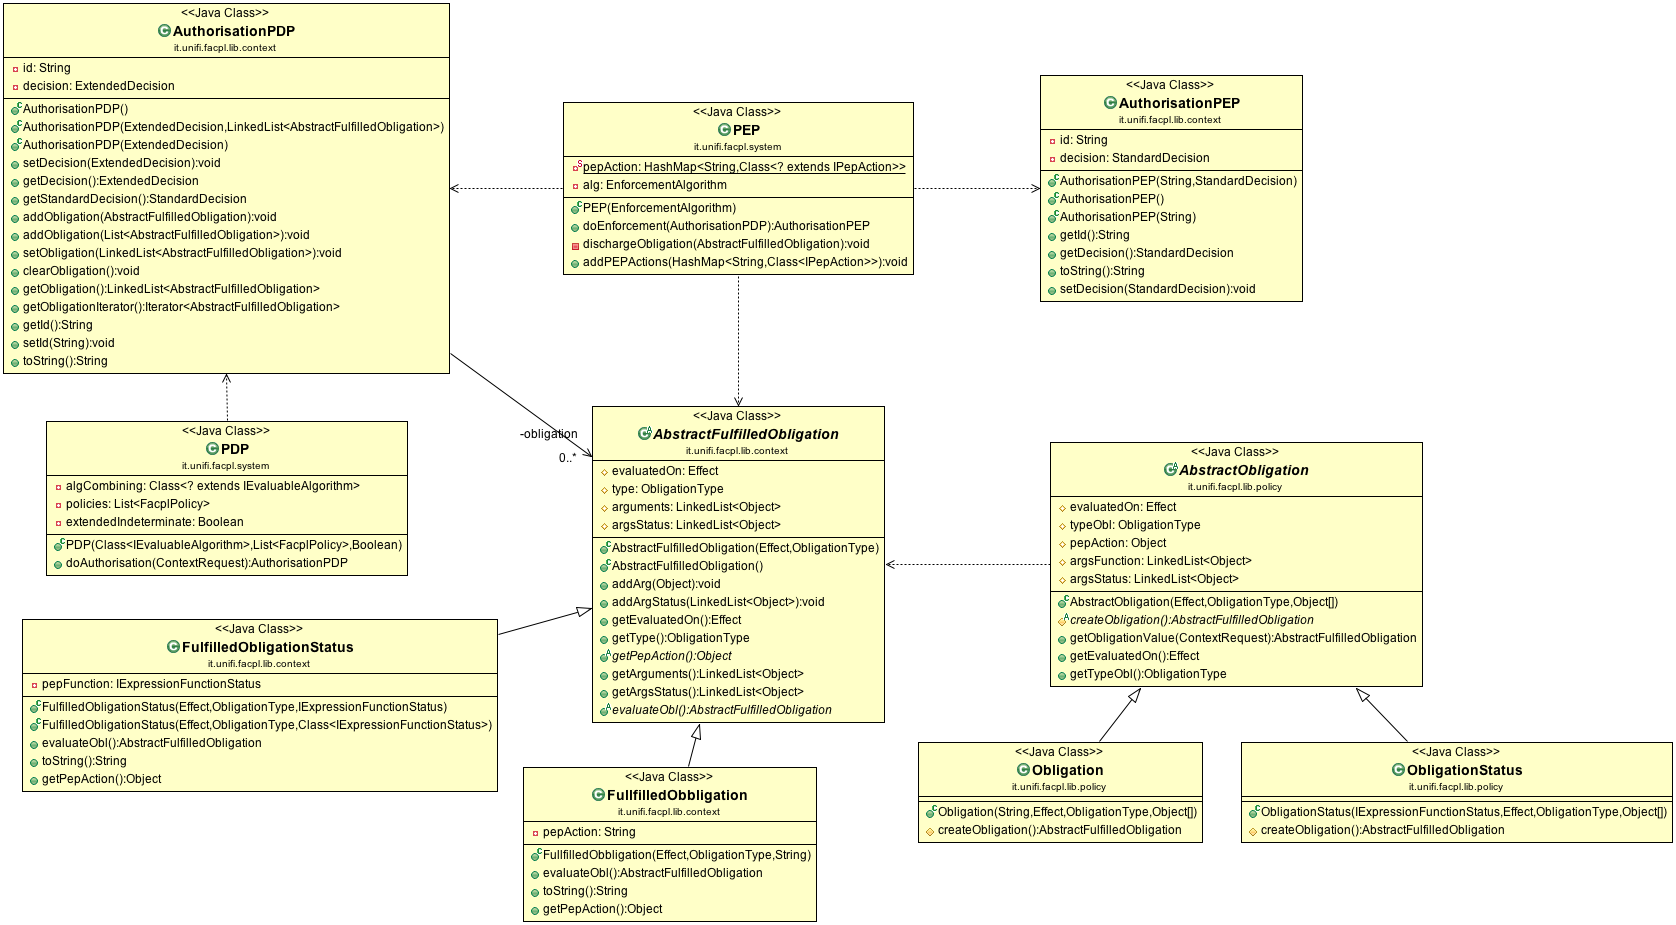
\includegraphics[width=1.1\linewidth]{obl.png}
    \caption{Relazioni tra Obligation e PEP}
    \label{fig:obl.png}
\end{sidewaysfigure}




\section{Plugin Eclipse}
\label{sec:plugin_eclipse}


[IN SOSPESO]


\section{Esempi}
\label{sec:implementazione_esempi}

In questa sezione 

\subsection{Primo case study}

\subsection{Secondo case study}